\chapter{Introduction}
\label{chapterIntro}
\section{Motivation}
Increasing data volumes in the field of genetics require sophisticated computational methods, since the bottleneck is no longer the data generation itself, but shifted notably towards the data analysis \cite{Forer2016}. The whole human genome with its size of over 3 billion positions can now be analyzed in short time with decreasing prices. Therefore the amount of data that has to be dealt with already increased and will so even more dramatically in future. Therefore, new algorithms and methods for data quality control (QC) are required, for increasing precision and recall to exceed currently available methods, in a scalable way. Misleading results can impact medical studies or forensic casework, where errors introduced by computational methods can have severe consequences. The focus of this work is on computational methods for reproducible QC of DNA from a small genome, contained in the mitochondria. Although its length contributes only to $0.0005\%$ to the complete human genome, high-throughput data is required to investigate processes still unclear, like the development of mutations and its fixation in cancer or processes on the mitochondrial DNA (further denoted as mtDNA) related with aging. This data generation makes it indispensable to process without scalable and reproducible pipelines. 
\\
\\
The human mitochondrial DNA, henceforth abbreviated as mtDNA, plays an important role in today's life-science and is of especial interest in the field of population genetics, forensics and clinical disease association studies. The mitochondrial DNA has some features (more to find in Chapter \ref{chap:BioFound}) that make it predestined for genealogists when it comes to creation of family trees but also helps forensics in identifying persons or victims even with degraded body remains, or clinicians to help investigating diseases, since bioenergetic aspects, where mitochondria are heavily involved, offer new opportunities for diagnosis and therapy \cite{Picard2016}.
The following issues and challenges need to be addressed in this context:
\begin{itemize}
\item 
Mitochondrial DNA can be classified into a natural grouping of sequence haplotypes; into so called haplogroups. These haplogroups play an important role in the area of phylogenetics, but also in data QC of mtDNA data. While the manual assignment of mtDNA profles to haplogroups is very time-consuming besides being error prone, the increase of data generated, require sophisticated automatic procedures to solve this task. Therefore an algorithm is required to assigning the closest haplogroup to mtDNA profiles based on a maximum parsimony tree present \cite{VanOven2009}. With classical sequencing devices the data generation of mtDNA profiles might seem straightforward, but it is also error prone. To determine and correct these data errors, methods are required to perform QC to highlight issues in mtDNA data. The growing sample sizes in various studies require methods with linear increase in computation time and memory consumption, to consider the increasing data. 
\item 
One of the most prominent problems in the field of bioinformatics is the alignment of sequences. The algorithms in this regard are known to have complexity of $\mathcal O(nm)$ where \textit{n} and \textit{m} represent the length of the sequences to be compared, leading to $\mathcal O(n^2)$ in both time and space. There exist optimization as well as data structures to face this problem, and might seem trivial for mtDNA with its size of less than $\sim$ 17kb \cite{Andrews1999}. However, in order to detect variants according the correct nomenclature, several rules need to be considered, sometimes contradicting, rendering it almost impossible to generate unambiguous alignments \cite{Bandelt2008}. Ambiguous alignments without assumptions from evolutionary perspectives, especially in low-complexity regions, can influence the haplogroup assignment, and could lead to misinterpretation of results.  
\item 
A further challenge for computational biologists and computer scientists is the establishment of next-generation sequencing (NGS) devices in the last years, producing literally big data. The management of such data is not feasible for relational databases, requiring new paradigms such as key-value based models like MapReduce \cite{Dean2008}. The mtDNA with it's small size is in contrast to the nuclear DNA a tiny genome sequence, but due to it's property, being present between 100 and several 1,000 fold per cell, it requires sequencing with high coverage. This exploitation of the massive parallel sequencing is required in order to get a deeper understanding in mitochondrial mutations. These mutations are often involved in diseases and poorly understood at this time \cite{Wallace2013}. Since the error rates of the new devices are higher than the former gold standard \cite{Wang2011}, additional QC-steps are required, to prevent the detection of false positive mutations. 

\end{itemize}

In this thesis, solutions to the drafted issues are proposed. Software tools, which can operate as stand-alone applications but also can be merged to one pipeline for contamination detection in NGS studies, are presented. Thereby the detection of contamination is not limited to pure mtDNA sequencing projects. By taking advantage of  mtDNA sequences in whole genome sequencing or whole exome sequencing projects, benefit of this approach for contamination detection. It represents a fast and straightforward method for quality control of MPS datasets prior to publication. Thereby mtDNA makes an intrinsic contamination control for whole genome sequencing projects available and highlights the merits of this underrated extra “chromosome” paired with computational methods. The scalable pipeline can handle large data sets of several hundred GBs as shown in the context of this work. 

\section{Preliminary Work}
\label{prelimWork}
This work is the continuation of an interdisciplinary cooperation between the group of Databases and Information Systems of the University of Innsbruck and the Department of Genetic Epidemiology at the Medical University of Innsbruck which started back in 2007 and led to my master's degree in computer science in 2008. Back then the focus was on the development of a database for genotype data (the blueprint of an organism, contained in each cell) and phenotype data (an organism's observed properties, such as the physical appearance like eye color or the body mass index, disease or behavior with the result published in BMC Bioinformatics \cite{Schoenherr2009}. This database was the foundation for the next project, which was to extend it for QC and further functionality to work with a special and very specific DNA from an organelle with its own genome, the mitochondrial genome. 
\\
Different methods for the generation of mtDNA data exist, as presented in section \ref{sec:dataGeneration}. While the data generation is getting increasingly more straightforward, the data management gets more complex. Checks for data quality are needed, to avoid the processing of false positive data, that could lead to misinterpretation of diseases, to wrong publications and conclusions or even to the arrest of innocent persons, just to show the severity these consequences can have in the different areas applied.
Therefore a short summary about this basic concept is presented here, that shows the mtDNA data management in a relational database. Since this system is based on a previous work by Sch\"onherr and Weissensteiner \cite{Schoenherr2009} from 2009, the database structure's concept is to store phenotypes in a key-value like schema (where a key has a value and a time-stamp), by implementing 3 different entities for each data-type $(STRING, INTEGER, DOUBLE)$.
\begin{figure}[ht]
\begin{center}
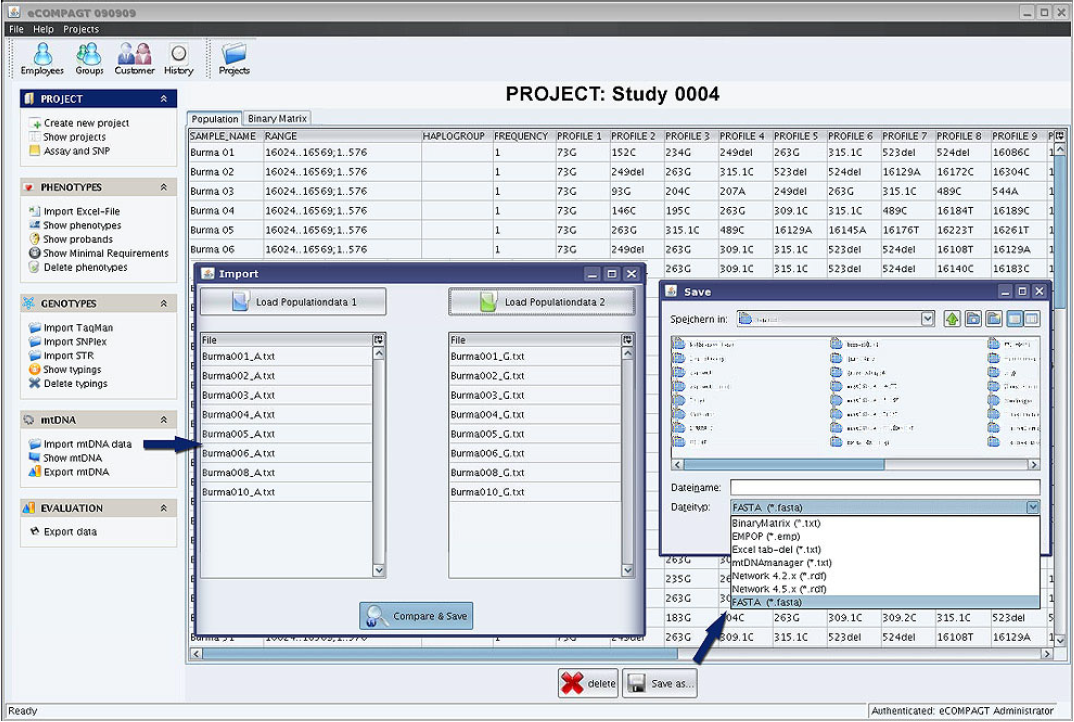
\includegraphics[scale=0.46]{ecompagt.png}
\caption[eCOMPAGTs User Interface]{eCOMPAGTs User Interface for mtDNA handling: the input data is checked for concordance, while several file exports are supported. Figure presented in Weissensteiner et al. \cite{Weissensteiner2010}}.
\label{fig:ecompagt}
\end{center}
\end{figure}
Both phenotypes and genotypes are stored in a previously IBM DB2 database, in an updated version also Oracle and MySQL relational database management systems are supported. When working with mtDNA data from sequencing devices, we integrated an workflow for the analysis in eCOMPAGT, to securely import, validate, store and export mtDNA profiles.  These can further be connected to phenotype data by using eCOMPAGT's combination and evaluation feature. Data import comprise data in EMPOP format \cite{Parson2007}, or from Sequencher/SeqScape mutation reports. Data Exports provide various formats for different applications: EMPOP as well as FASTA files, file for generation of phylogenetic networks in Network.exe\footnote{\url{fluxus-engineering.com}}  \cite{Bandelt1999}, mtdnaManager\cite{Lee2008}, as well as HaploGrep input files \cite{Kloss-Brandstatter2011,Weissensteiner2016a}. Figure \ref{fig:ecompagt} shows the graphical user interface of the database, based on Java Swing and SwingX. The workflow, as well as the underlying architecture are not further presented in this work, I refer to the publications by Sch\"onherr and Weissensteiner \cite{Schoenherr2009,Weissensteiner2010}. These articles build the groundwork of the subsequently research effort. One previously identified limitation of this system is addressed and solved in the the subsequenct Chapter \ref{chapterHaplogrep}, by presenting HaploGrep.

\section{Problem characterization}
\label{sect:ProblChar}
The aim of this work is to propose an information management system for mtDNA data. 
The most common input formats from Sanger based Sequencing, over genotyping data from MicroArrays to the Next-Generation Sequencing for mitochondrial DNA  are covered and merged into a management system for quality control. Sample contamination is still a severe problem, not only for anthropologists dealing with degraded mtDNA but for all types of areas dealing with mtDNA (forensics, medical genetics, population genetics). With new technologies, contamination detectable due to the high resolution of genomes, becomes a new issue in the lab, and requires control mechanisms in data post-processing. Therefore quality control based on the mitochondrial DNA haplogroups is essential for both Sanger Sequencing as well as for Next-Generation-Sequencing and will play a major role in this thesis. Within the next Chapter \ref{chap:BioFound} Biological Background, the basic features of mtDNA, as well as the data formats are presented. An already implemented database for mtDNA data were presented (Publications in BMC Bioinformatics \cite{Schoenherr2009}, \cite{Weissensteiner2010}) as drafted in \ref{prelimWork}, able to perform basic QC steps only.

The core purpose of this investigation was to build an information system for managing data from the often so called powerhouses of the cell, the mitochondria with their own mitochondrial DNA. Besides the initial database (see \ref{prelimWork}, several additional algorithms and frameworks which all can be connected to a pipeline and as a matter of fact are connected in Chapter \ref{chap:NGS} and Chapter \ref{chapterContamination} yield to high-quality mtDNA data. The herein developed JAVA based software solutions are abstracted in the next paragraphs and are presented in detail in the corresponding chapters.

Chapter \ref{chapterHaplogrep} describes the foundations of mitochondrial classification to haplogroups based on an XML tree. Several binary similarity and distance measures are evaluated and our solution HaploGrep is compared to related work. \\

Chapter \ref{chap:alignment} deals with the theoretical background as well as the JAVA implementation for aligning mitochondrial genome data efficiently as an extension to chapter \ref{chapterHaplogrep}, and are presented as part of the subsequent publication. As data volume increases with Next-Generation Sequencing, a MapReduce based approach is presented in chapter \ref{chap:NGS} to sequence the mitochondrial genome with a high coverage, resulting in computational intensive mapping of the short-reads to the reference sequence. 
\\
The resulting profiles yield insights in heteroplasmy levels and are an indication for data quality by applying an haplogroup discordance check presented in chapter \ref{chapterContamination}. Based on this check contamination not only in targeted mtDNA sequencing studies, but also in Whole Genome and Whole Exome Sequencing Projects can be detected. This approach is partly presented in Weissensteiner et al. \cite{Weissensteiner2016b} and is part of a work that is currently prepared for publication. Figure \ref{fig:figureBigPic} gives an overview of the chapters represented in this work and their relation as a schematic software stack.
\\ 
The chapter \ref{chap:conclusion} finally gives a summary of the different key aspects, shows strengths and limitations of our pipeline while Chapter \ref{outlook} gives an outlook of possible optimization and on future work.

\begin{figure}[ht]
\begin{center}
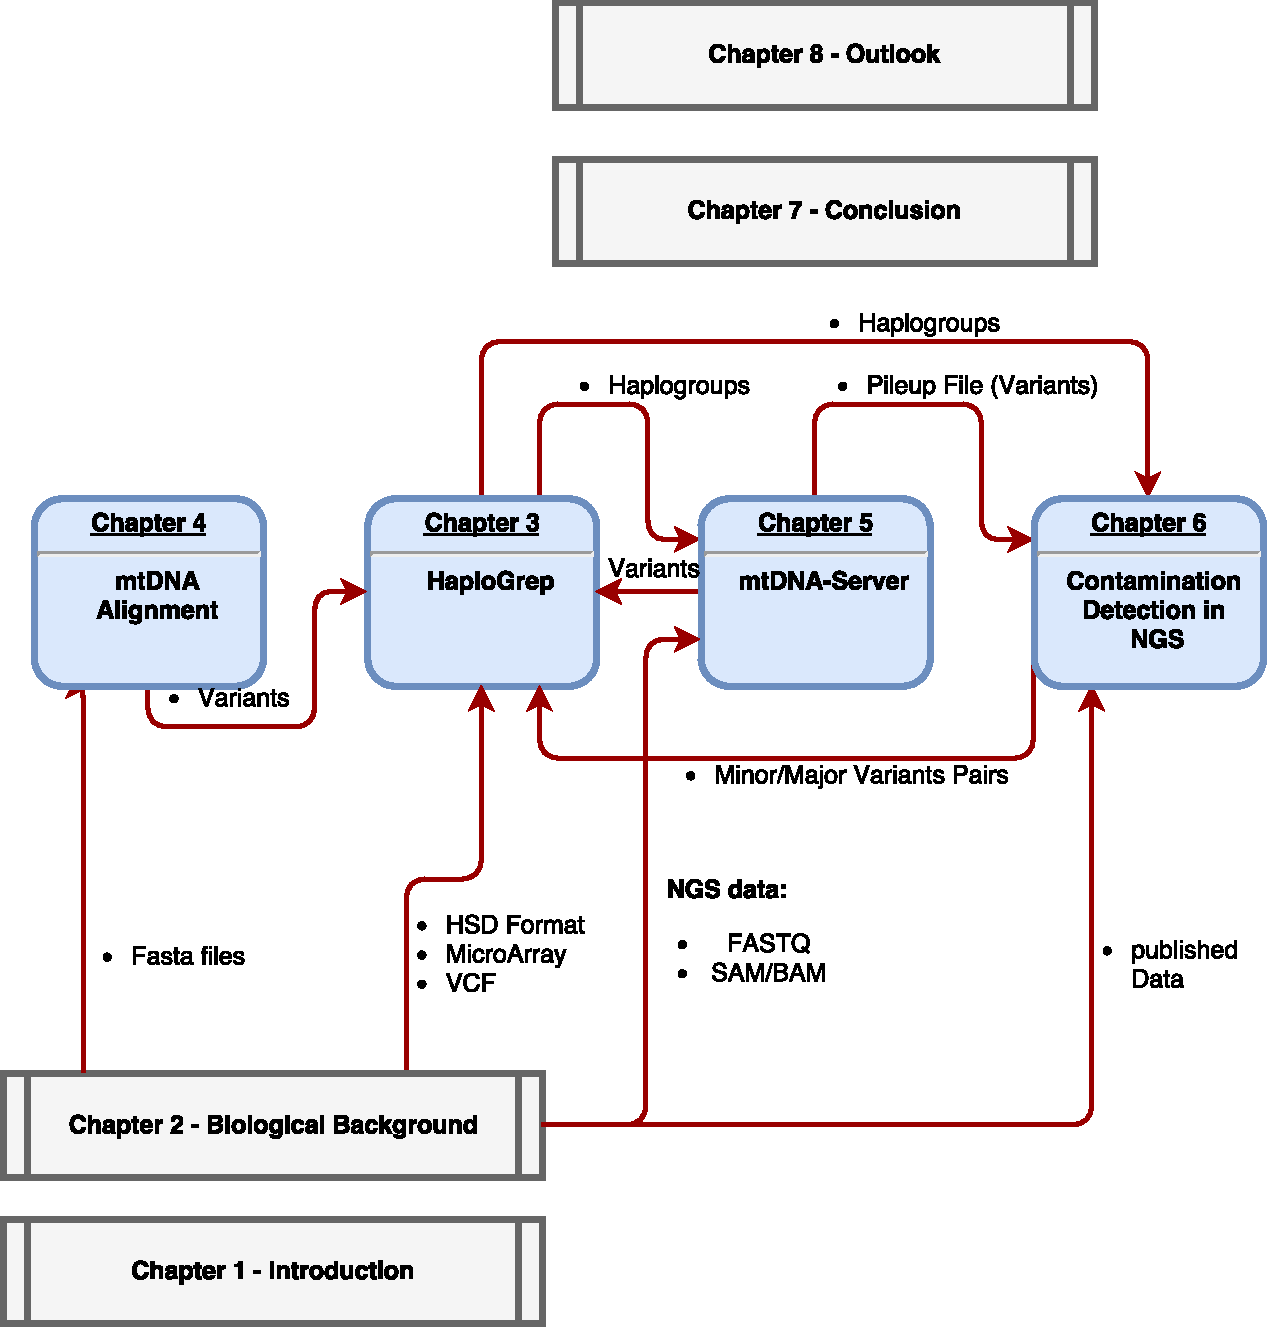
\includegraphics[scale=0.5]{BigPicture.pdf}
\caption[Representation of chapters]{Representation of chapters and their connection to a contamination detection method, covering various file formats }
\label{fig:figureBigPic}
\end{center}
\end{figure}

\section{Research Aims and Contribution}
Research demands collaboration. This work is largely the result of collaboration with computer scientists, programmers, database experts, biologists, mathematicians, medical doctors, medical technical assistants and many more. It is in fact interdisciplinary, as it is for genetics and genomics in general. Given the growing data generated with new sequencing devices, it is not feasible to process the data without a reproducible system, that takes the technical hurdles from the end user. Therefore the research aim is on providing sophisticated methods to the biologists, in such a manner that a problem can be solved by hiding the complexity from the user. Here it is mostly related with the handling of mtDNA data, where the end users have different background. The subsequent chapters represent some of the main work over several years of daily work with mtDNA data, highlighting the main contributions as drafted, resulting in several publications. 

The result presented in Chapter \ref{chapterHaplogrep} was published in Kloss-Brandst\"atter et al with shared first authorship in the journal Human Mutation \cite{Kloss-Brandstatter2011} and the successive extensions and optimizations were published in Weissensteiner et al presenting HaploGrep 2 in the 2016 Web Server Issue\footnote{\url{http://nar.oxfordjournals.org/content/44/W1.toc}} of Nucleic Acids Research\cite{Weissensteiner2016a}.

The work presented in Chapter \ref{chap:NGS} was also accepted in the 2016 Web Server Issue of Nucleic Acids Research in Weissensteiner et al \cite{Weissensteiner2016b} (acceptance quote of 31\%, see Editorial\footnote{\url{http://nar.oxfordjournals.org/content/44/W1/W1.full}}).

These published applications helped subsequent research questions, that led to further contributions in various publications (see Curriculum Vitae for full list of contributions), the most related with this work are the results in Summerer et al 2014 published in BMC Evolutionary Biology, \cite{Summerer2014} where we analyzed the mtDNA of 327 donors from Myanmar by considering the migration and generated phylogenetic trees identifying novel clusters. 

In a further work published in the Proceedings of the National Academy of Sciences \cite{Kehdy2015}, we analyzed the mtDNA data from 6,487 individuals, confirming the low native-american ancestry after european conquest, and shedding light on the African diaspora, where Brazil was a major destination.

The foundations for mtDNA-Server (Chapter \ref{chap:NGS} derived from two research projects: the MapReduce Framework Cloudgene \cite{Schonherr2012}, which we published in BMC Bioinformatics in 2012 and the Cancer Study of 28 individuals, where we compared different tissues in oral squamous cell carcinoma \cite{Kloss-Brandstatter2015}, by comparing Sanger based Sequencing to Next-Generation Sequencing, and showed that heteroplasmy detection down to the 1\% level is feasible with the new devices and the herein presented Apache Hadoop based approach. 

The further development of Cloudgene led to subsequent publication of Cloudflow in  2015 \cite{Forer2015} and 2016 \cite{Forer2016} respectively. Herein the Framework was extended not only to support Apache Hadoop with MapReduce but also Apache Spark pipelines. 

Several topics outside the mtDNA-field were also addressed in the recent years, leading to publications in the various peer-review journals like \textit{PLOS ONE} \cite{Weissensteiner2013} by describing SNPflow, a JAVA based application with an Ext-JS JavaScript user interface, an embedded Apache Tomcat server and MySQL-database for QC of genotype data derived by multiplex genotyping platforms. 

In the journal \textit{Atherosclerosis} we described a risk score for cardiovascular disease\cite{Lamina2014} implemented in JavaScript, and presented various works related to the relative telomere length \cite{Raschenberger2015assoc,Raschenberger2015dotelomeres}, in the German Chronic Kidney Disease (GCKD) study.

Lately, by modifying mtDNA-Server to work with different reference sequences, we were able to identify novel variants in a so far still unresolved highly repetitive region on the nuclear DNA, in the LPA gene, associated with cardiovascular disease \cite{Kronenberg2014}. The work is currently in press in the \textit{European Heart Journal} \cite{Coassin2017}. 


The work for the GCKD study lead to a membership of the consortium. As of February 2017 a membership in a consortium lead by the Max-Planck Institute for the Science of Human History was added.

Several conferences and workshops were attended in the last years (see CV), including venues in Qatar, USA, UK, Netherlands, Croatia, Germany and Austria, mostly in context of mtDNA data analysis. 


% \textit{2016}{H Weissensteiner et al. \textbf{mtDNA-Server: next-generation sequencing data analysis of human mitochondrial DNA in the cloud}, \textit{Nucleic Acids Research - Web Server Issue 2016}}
% \textit{2016}{H Weissensteiner et al. \textbf{HaploGrep 2: mitochondrial haplogroup classification in the era of high-throughput sequencing}, \textit{Nucleic Acids Research - Web Server Issue 2016}}
% \textit{2016}{L Forer et al. \textbf{Cloudflow-enabling faster biomedical pipelines with MapReduce and Spark}, \textit{Scalable Computing: Practice and Experience}}
% \textit{2015}{J Raschenberger et al. \textbf{Association of relative telomere length with cardiovascular disease in a large chronic kidney disease cohort: The GCKD study}, \textit{Atherosclerosis}}
% \textit{2015}{J Raschenberger et al. \textbf{Do telomeres have a higher plasticity than thought? Results from the German chronic kidney disease (GCKD) study as a high-risk population}, \textit{Experimental gerontology}}{}
% \textit{2015}{A Kloss-Brandst{\"a}tter et al. \textbf{Validation of Next-Generation Sequencing of Entire Mitochondrial Genomes and the Diversity of Mitochondrial DNA Mutations in Oral Squamous Cell Carcinoma}, \textit{PloS One}}
% \textit{2015}{FSG Kehdy et al. \textbf{Origin and dynamics of admixture in Brazilians and its effect on the pattern of deleterious mutations}, \textit{Proceedings of the National Academy of Sciences}}
% \textit{2015}{L Forer et al. \textbf{Cloudflow-A framework for MapReduce pipeline development in Biomedical Research}, \textit{Information and Communication Technology, Electronics and Microelectronics (MIPRO)}}
% \textit{2014}{ C Lamina et al. \textbf{Correlation between a positive family risk score and peripheral artery disease in one case-control and two population-based studies}, \textit{Atherosclerosis}}
% \textit{2014}{L Forer et al. \textbf{Delivering bioinformatics MapReduce applications in the cloud}, \textit{Information and Communication Technology, Electronics and Microelectronics (MIPRO)}}
% \textit{2014}{M Summerer et al. \textbf{Large-scale mitochondrial DNA analysis in Southeast Asia reveals evolutionary effects of cultural isolation in the multi-ethnic population of Myanmar}, \textit{BMC Evolutionary Biology}}
% \textit{2013}{ H Wei{\ss}ensteiner et al. \textbf{SNPflow: a lightweight application for the processing, storing and automatic quality checking of genotyping assays}, \textit{Plos One}}
% \textit{2012}{ S Sch\"onherr et al. \textbf{Cloudgene: A graphical execution platform for MapReduce programs on private and public clouds}, \textit{BMC Bioinformatics}}
% \textit{2012}{L Forer et al. \textbf{Cloud Computing}, \textit{Book Chapter: Computational Medicine}}
% \textit{2011}{S Sch\"onherr et al. \textbf{A feedback guided interface for elastic computing}, \textit{Grundlagen von Datenbanken}}
% \textit{2010}{A Kloss-Brandst{\"a}tter et al. \textbf{HaploGrep: a fast and reliable algorithm for automatic classification of mitochondrial DNA haplogroups}, \textit{Human mutation}}
% \textit{2010}{L Forer et al. \textbf{CONAN: copy number variation analysis software for genome-wide association studies}, \textit{BMC Bioinformatics}}{}
% \textit{2010}{H Wei{\ss}ensteiner et al. \textbf{eCOMPAGT integrates mtDNA: import, validation and export of mitochondrial DNA profiles for population genetics, tumour dynamics and genotype-phenotype association studies}, \textit{BMC Bioinformatics}}
% \textit{2009}{S Sch\"onherr et al. \textbf{eCOMPAGT - efficient combination and management of phenotypes and genotypes for genetic epidemiology}, \textit{BMC Bioinformatics}}
